%% This is file `elsarticle-template-1-num.tex',
%%
%% Copyright 2009 Elsevier Ltd
%%
%% This file is part of the 'Elsarticle Bundle'.
%% ---------------------------------------------
%%
%% It may be distributed under the conditions of the LaTeX Project Public
%% License, either version 1.2 of this license or (at your option) any
%% later version.  The latest version of this license is in
%%    http://www.latex-project.org/lppl.txt
%% and version 1.2 or later is part of all distributions of LaTeX
%% version 1999/12/01 or later.
%%
%% The list of all files belonging to the 'Elsarticle Bundle' is
%% given in the file `manifest.txt'.
%%
%% Template article for Elsevier's document class `elsarticle'
%% with numbered style bibliographic references
%%
%% $Id: elsarticle-template-1-num.tex 149 2009-10-08 05:01:15Z rishi $
%% $URL: http://lenova.river-valley.com/svn/elsbst/trunk/elsarticle-template-1-num.tex $
%%
%\documentclass[preprint,12pt]{elsarticle}

%% Use the option review to obtain double line spacing
\documentclass{elsarticle}

%% Use the options 1p,twocolumn; 3p; 3p,twocolumn; 5p; or 5p,twocolumn
%% for a journal layout:
%% \documentclass[final,1p,times]{elsarticle}
%% \documentclass[final,1p,times,twocolumn]{elsarticle}
%% \documentclass[final,3p,times]{elsarticle}
%% \documentclass[final,3p,times,twocolumn]{elsarticle}
%% \documentclass[final,5p,times]{elsarticle}
%% \documentclass[final,5p,times,twocolumn]{elsarticle}

%% if you use PostScript figures in your article
%% use the graphics package for simple commands
%% \usepackage{graphics}
%% or use the graphicx package for more complicated commands
%% \usepackage{graphicx}
%% or use the epsfig package if you prefer to use the old commands
%% \usepackage{epsfig}

%% The amssymb package provides various useful mathematical symbols
\usepackage{bibentry}
%% The amsthm package provides extended theorem environments
% packages added by Vahid
\usepackage{changes}
\definechangesauthor[name=YS,color=brown]{YS}
\definechangesauthor[name=MM,color=blue]{MM}
%\usepackage{tablefootnote}
\usepackage{amssymb, bm, mathrsfs, xcolor, hyperref}
\usepackage{hyperref}
\usepackage{comment}
\usepackage{amsthm}
\usepackage{amsmath,amssymb,bm}
\usepackage{stmaryrd}
\usepackage[boxed]{algorithm2e}
\usepackage{subfig}
 \usepackage[mathscr]{euscript}
%\usepackage{xcolor}
\usepackage{blindtext, xcolor}
%\usepackage{showlabels}
%\newcommand{\todo}[1]{{\color{red} #1}}
\usepackage{todonotes}
\newcommand{\Comment}[1]{{\color{blue}\vspace{5 mm}\par \noindent
  \marginpar{\textsc{Comment}} \framebox{\begin{minipage}[c]{0.95
        \textwidth} \tt #1 \end{minipage}}\vspace{5 mm}\par}}
\newcommand{\review}[1]{ \textit{#1}}

%\newcommand{\comment}[1]
%{\par {\bfseries \color{blue} #1 \par}}

%% The lineno packages adds line numbers. Start line numbering with
%% \begin{linenumbers}, end it with \end{linenumbers}. Or switch it on
%% for the whole article with \linenumbers after \end{frontmatter}.
%% \usepackage{lineno}

%% natbib.sty is loaded by default. However, natbib options can be
%% provided with \biboptions{...} command. Following options are
%% valid:

%%   round  -  round parentheses are used (default)
%%   square -  square brackets are used   [option]
%%   curly  -  curly braces are used      {option}
%%   angle  -  angle brackets are used    <option>
%%   semicolon  -  multiple citations separated by semi-colon
%%   colon  - same as semicolon, an earlier confusion
%%   comma  -  separated by comma
%%   numbers-  selects numerical citations
%%   super  -  numerical citations as superscripts
%%   sort   -  sorts multiple citations according to order in ref. list
%%   sort&compress   -  like sort, but also compresses numerical citations
%%   compress - compresses without sorting
%%
%% \biboptions{comma,round}

% \biboptions{}


\journal{Journal of Natural Gas Science and Engineering}
\graphicspath{
  {./figures/}}

\DeclareMathOperator{\divergence}{div}

\DeclareMathOperator{\sign}{sign}

\begin{document}

\begin{frontmatter}

%% Title, authors and addresses

%% use the tnoteref command within \title for footnotes;
%% use the tnotetext command for the associated footnote;
%% use the fnref command within \author or \address for footnotes;
%% use the fntext command for the associated footnote;
%% use the corref command within \author for corresponding author footnotes;
%% use the cortext command for the associated footnote;
%% use the ead command for the email address,
%% and the form \ead[url] for the home page:
%%
%% \title{Title\tnoteref{label1}}
%% \tnotetext[label1]{}
%% \author{Name\corref{cor1}\fnref{label2}}
%% \ead{email address}
%% \ead[url]{home page}
%% \fntext[label2]{}
%% \cortext[cor1]{}
%% \address{Address\fnref{label3}}
%% \fntext[label3]{}

\title{Response to reviewer comments on `Numerical modeling of CO$_2$ fracturing by the phase field approach'}

%% use optional labels to link authors explicitly to addresses:
%% \author[label1,label2]{<author name>}
%% \address[label1]{<address>}
%% \address[label2]{<address>}

\author[mymainaddress]{Mostafa Mollaali}
%\ead[url]{www.elsevier.com}

\author[mysecondaryaddress]{Vahid Ziaei-Rad}
%\ead[url]{www.elsevier.com}

\author[mymainaddress]{Yongxing Shen\corref{mycorrespondingauthor}}
\cortext[mycorrespondingauthor]{Corresponding author}
\ead{yongxing.shen@sjtu.edu.cn}

\address[mymainaddress]{University of Michigan -- Shanghai Jiao Tong University Joint Institute, Shanghai Jiao Tong University,	Shanghai, 200240, China}
\address[mysecondaryaddress]{Department of Civil Engineering, Isfahan University of Technology, Isfahan 84156-83111, Iran}
\end{frontmatter}

%%
%% Start line numbering here if you want
%%
% \linenumbers

%% main text
We thank the reviewers again for their constructive comments. Below we respond to each of the comments, along with the corresponding changes of the manuscript. All changes to the previous submission are marked {\color{blue} in blue} in the revised version.


%----------------------------------------------------------------------------------------------------

\section*{Comments from Reviewer \#2}

\review{To the best of my knowledge, the proposed method is novel and the paper is well written. All my questions have been answered in this revision. From my opinion, this paper is acceptable for publication without further revision.}
\bigskip

%{We appreciate the reviewer's positive comment.}
%
%\bigskip

%-------------------------------------------------------------------------------------
\section*{Comments from Reviewer \#3}
    \review{The modification does not solve my major concerns.}
\bigskip

	\review{1. Regarding Question 4: Mandel's problem is a typical poroelastic problem. It is not for incompressible fluid. The principles behind the poroelastic borehole are the same as those in the Mandel's problem. The authors did not demonstrated typical poroelastic response through borehole pressurization.}
	\bigskip
	
%	\todo[inline,author=YS]{Why not start with positive points that we have done a certain analysis on Mandel's problem?\\ Vahid: I startetd with Mandel's problem, and at the end I explained why we did not include this example into the manuscript.}
	
We did try to solve Mandel's problem with our algorithm, and the results are satisfactory. Nevertheless, we do not plan to include it in the manuscript, because in some sense it repeats the numerical example in Section 4.2, as both couple porous flow and the displacement of the porous medium.
	
	In the sequel, we first describe how we solved Mandel's problem with our algorithm.
	Consider a 2D rectangular domain of width $2a$ and height $2b$ occupied by a saturated poroelastic material. Constant compression forces are applied on rigid impermeable plates $y=\pm b$ with a magnitude of $2F$, see the configuration in Figure \ref{Fig:mandel}. The load is applied instantaneously at $t=0^+$. At the right edge ($x = \pm a$) the sample can be drained while the lateral boundaries are free of stress.
	
	%The governing equations for modeling the CO$_2$ fracturing are summarized as follow: for the porous medium deformation, the functional defined in (3) is minimized among $(\bm{u},d)\in \mathscr{S}_u\times\mathscr{S}_d$ under the constraint (5), while for the compressible fluid the boundary value problem (13) is used to solve for the pressure $p$. Also, we use fixed stress splitting method $\cdots$.
	
	We only model a quarter of the sample due to symmetry. The sample is assumed to be under plane strain conditions. The following boundary conditions are imposed:
	\begin{eqnarray*}
	p=0 \quad &\text{on}  \quad x=a, \\
	u_2=U_2(b,t) \quad &\text{on}\quad y=b,\\
	u_1=0 \quad &\text{on} \quad x=0,\\
	u_2=0 \quad &\text{on} \quad y=0.
	\end{eqnarray*}
where $U_2(b,t))$ is the value of Mandel's closed form solution at $y =  b$ [Y.~Abousleiman, A.-D.~Cheng, L.~Cui, E.~Detournay, J.-C.~Roegiers, Mandel's problem revisited, Geotechnique 46 (2) (1996) 187–195].
The remaining boundary conditions are traction free boundary conditions.

	%\todo[inline,author=YS]{What is $U_2$?\\MM:The definition of $U_2(b,t)$ is added.}
	
	%In this case, we use the Mandel analytical solutions \cite{mandel1953consolidation} to make comparisons numerical solutions. The analytical pore pressure  during the consolidation stage is as follows
	
%	\begin{equation*}
%	p(x,t)=\dfrac{2FB(1+\nu_u)}{3a} \sum^{\infty}_{i=1} \dfrac{sin ~\alpha_i}{\alpha_i-sin ~\alpha_i cos~ \alpha_i}\left(cos~\frac{\alpha_i x}{a}-cos~\alpha_i \right)exp~\left(-\alpha_i^2ct/a^2 \right)  
%	\end{equation*}
%	where
%	\begin{equation*}
%	c=\dfrac{2kB^2G(1-\nu)(1+\nu_u)^2}{9\mu(1-\nu_u)(\nu_u-\nu)},
%	\end{equation*}
%	
%	\begin{equation*}
%	tan ~\alpha_i=\dfrac{1-\nu}{\nu_u-\nu} \alpha_i.
%	\end{equation*}
	
	Based on the analytical solution, as the compression load $2F$ is imposed, an instantaneous pressure increase and the following deformation responses are expected:	
	\begin{eqnarray*}
		p(x, y, 0^+) &=&\dfrac{FB(1+\nu_u)}{3a},\\
		u_1(a, y, 0^+) &=&\dfrac{F\nu_u}{2G},\\
		u_2(x, b, 0^+) &=&-\dfrac{Fb(1-\nu_u)}{2Ga}.
	\end{eqnarray*}
	
	\begin{figure}[htbp]
		\centering
		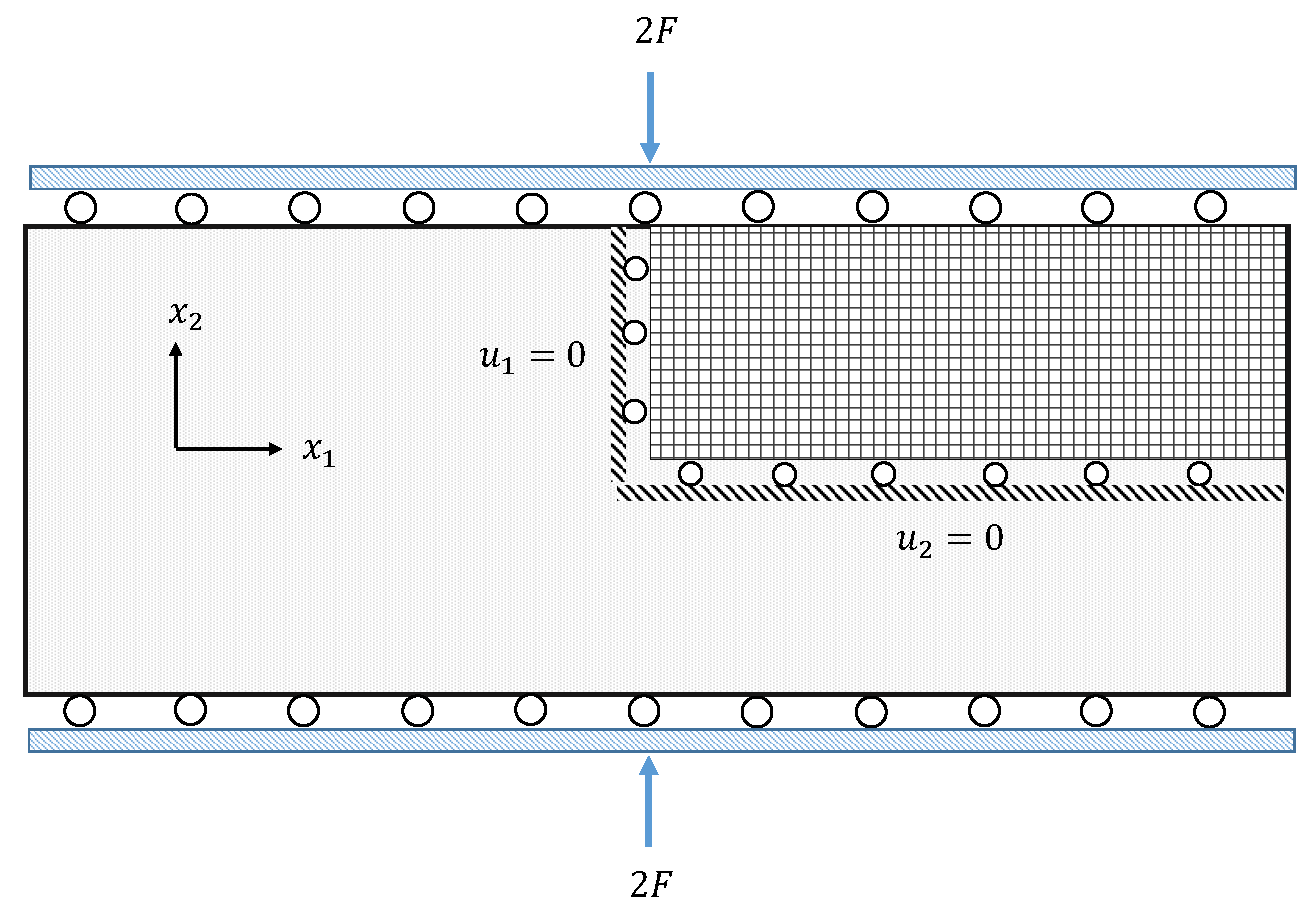
\includegraphics[width=0.8\textwidth]{MANDEL}
		\caption{Schematic view of Mandel's problem. An instantaneous compression force $2F$ is applied on the horizontal edges. Due to symmetry, only a quarter of the sample is modeled with proper boundary conditions.}
		\label{Fig:mandel}
	\end{figure}
	
%\todo[inline,author=YS]{Figure \ref{Fig:mandel_snapshots} is not referenced.\\MM:Done}
	
	The material parameters for rock and fluid are given in Table \ref{Tab:Mandel_input}. Using our proposed algorithm in combination with the fixed-stress split method (see [43][44], which we have now also cited in the manuscript, see Section 3), we solved the numerical problem for $t_f=6$s in 600 equal time steps. Figure \ref{Fig:mandel_pressure} shows our numerical results and the analytical solution for pore pressure. Excellent agreement is observed. Figure \ref{Fig:mandel_snapshots} shows the pore pressure developed in the sample during consolidation.
	
		\begin{table}[htbp]
		\centering
		\caption{Mandel's problem: Input parameters according to [43].}
		\begin{tabular}{l c c c}
			\hline 
			Parameters & symbol & unit& value \\
			\hline 
			Young's modulus & $E$ &MPa&  1\\
			Poisson's ratio & $\nu$ &$-$&  0.2\\
			Biot coefficient & $\alpha$ &$-$&  1.\\
			Permeability & $k_0$ &m$^2$&  1\\
			Viscosity &$\mu$ & MPa$\cdot$s &  1\\
			Length & $a$ & m &  2.5\\
			Height & $b$ & m &  1\\
			Load&$F$& MN& 2.5\\     
			Skempton coefficient &$B$& $-$& 1\\                    
			Drained Poisson's ratio&$\nu_u$& $-$&  0.5\\      
			Biot's modulus  & M & MPa & $\infty$ \\                                               
			\hline      
		\end{tabular}
		\label{Tab:Mandel_input}
	\end{table}
	
	
	\begin{figure}[htbp]
		\centering
		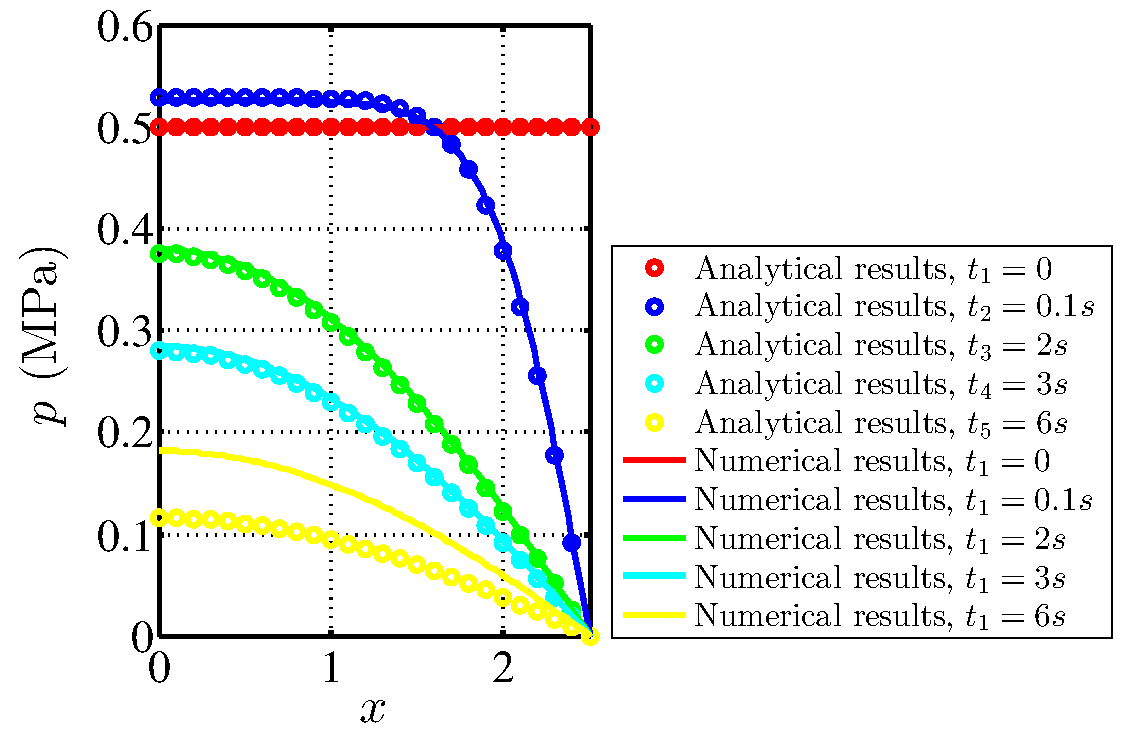
\includegraphics[width=0.8\textwidth]{mandel_pressure}
		\caption{Mandel's problem: change of pore pressure in time. Excellent agreement is observed with the analytical solution.}
		\label{Fig:mandel_pressure}
	\end{figure}
	
	\begin{figure}[]
		\centering %
		\subfloat[]{
\includegraphics[width=80mm]{t9}\label{Fig:mandel_t_9}}
		\\
		\subfloat[]{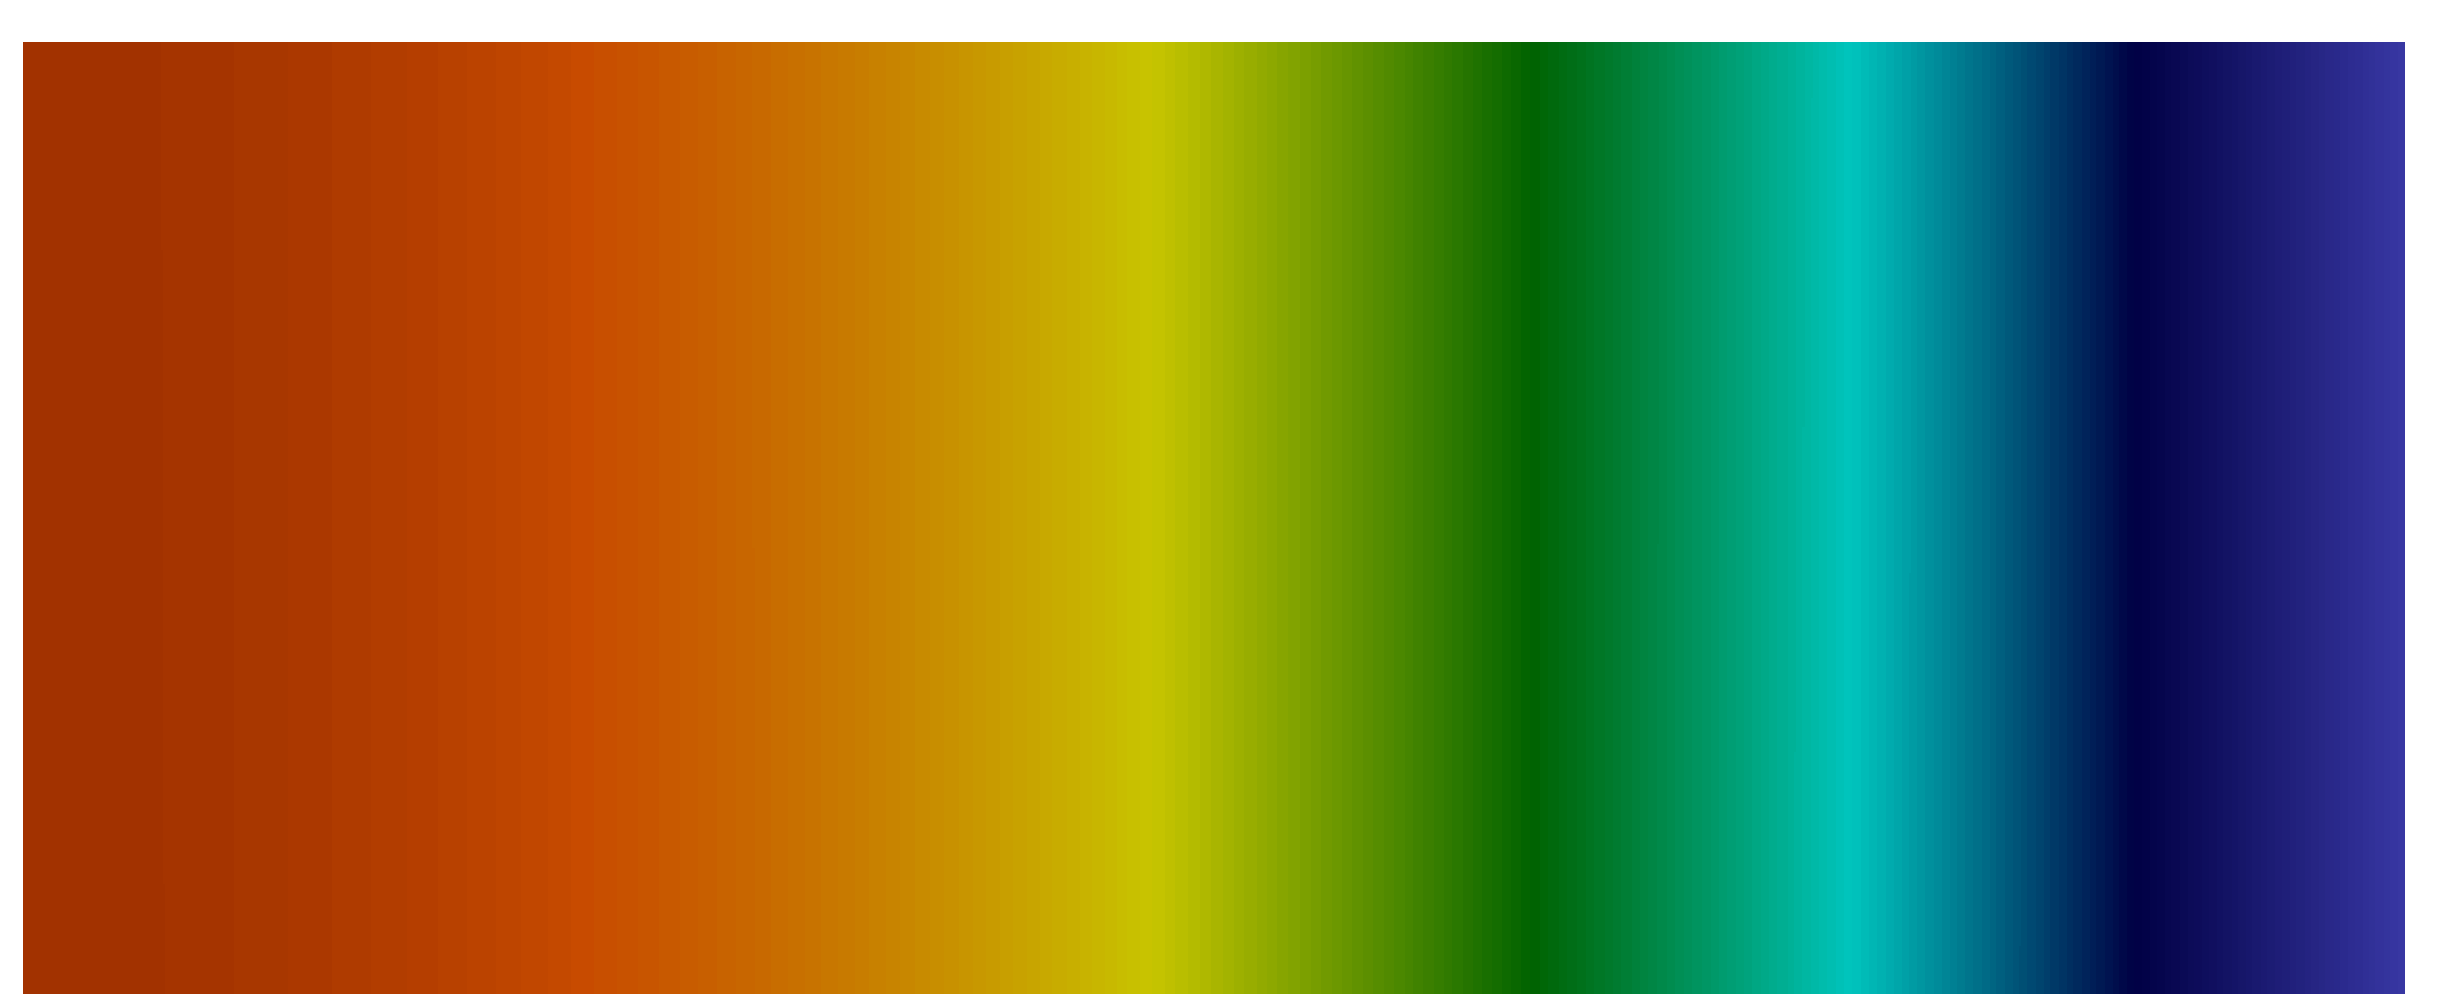
\includegraphics[width=80mm]{t199}\label{Fig:mandel_t_199}}
		\\
		\subfloat[]{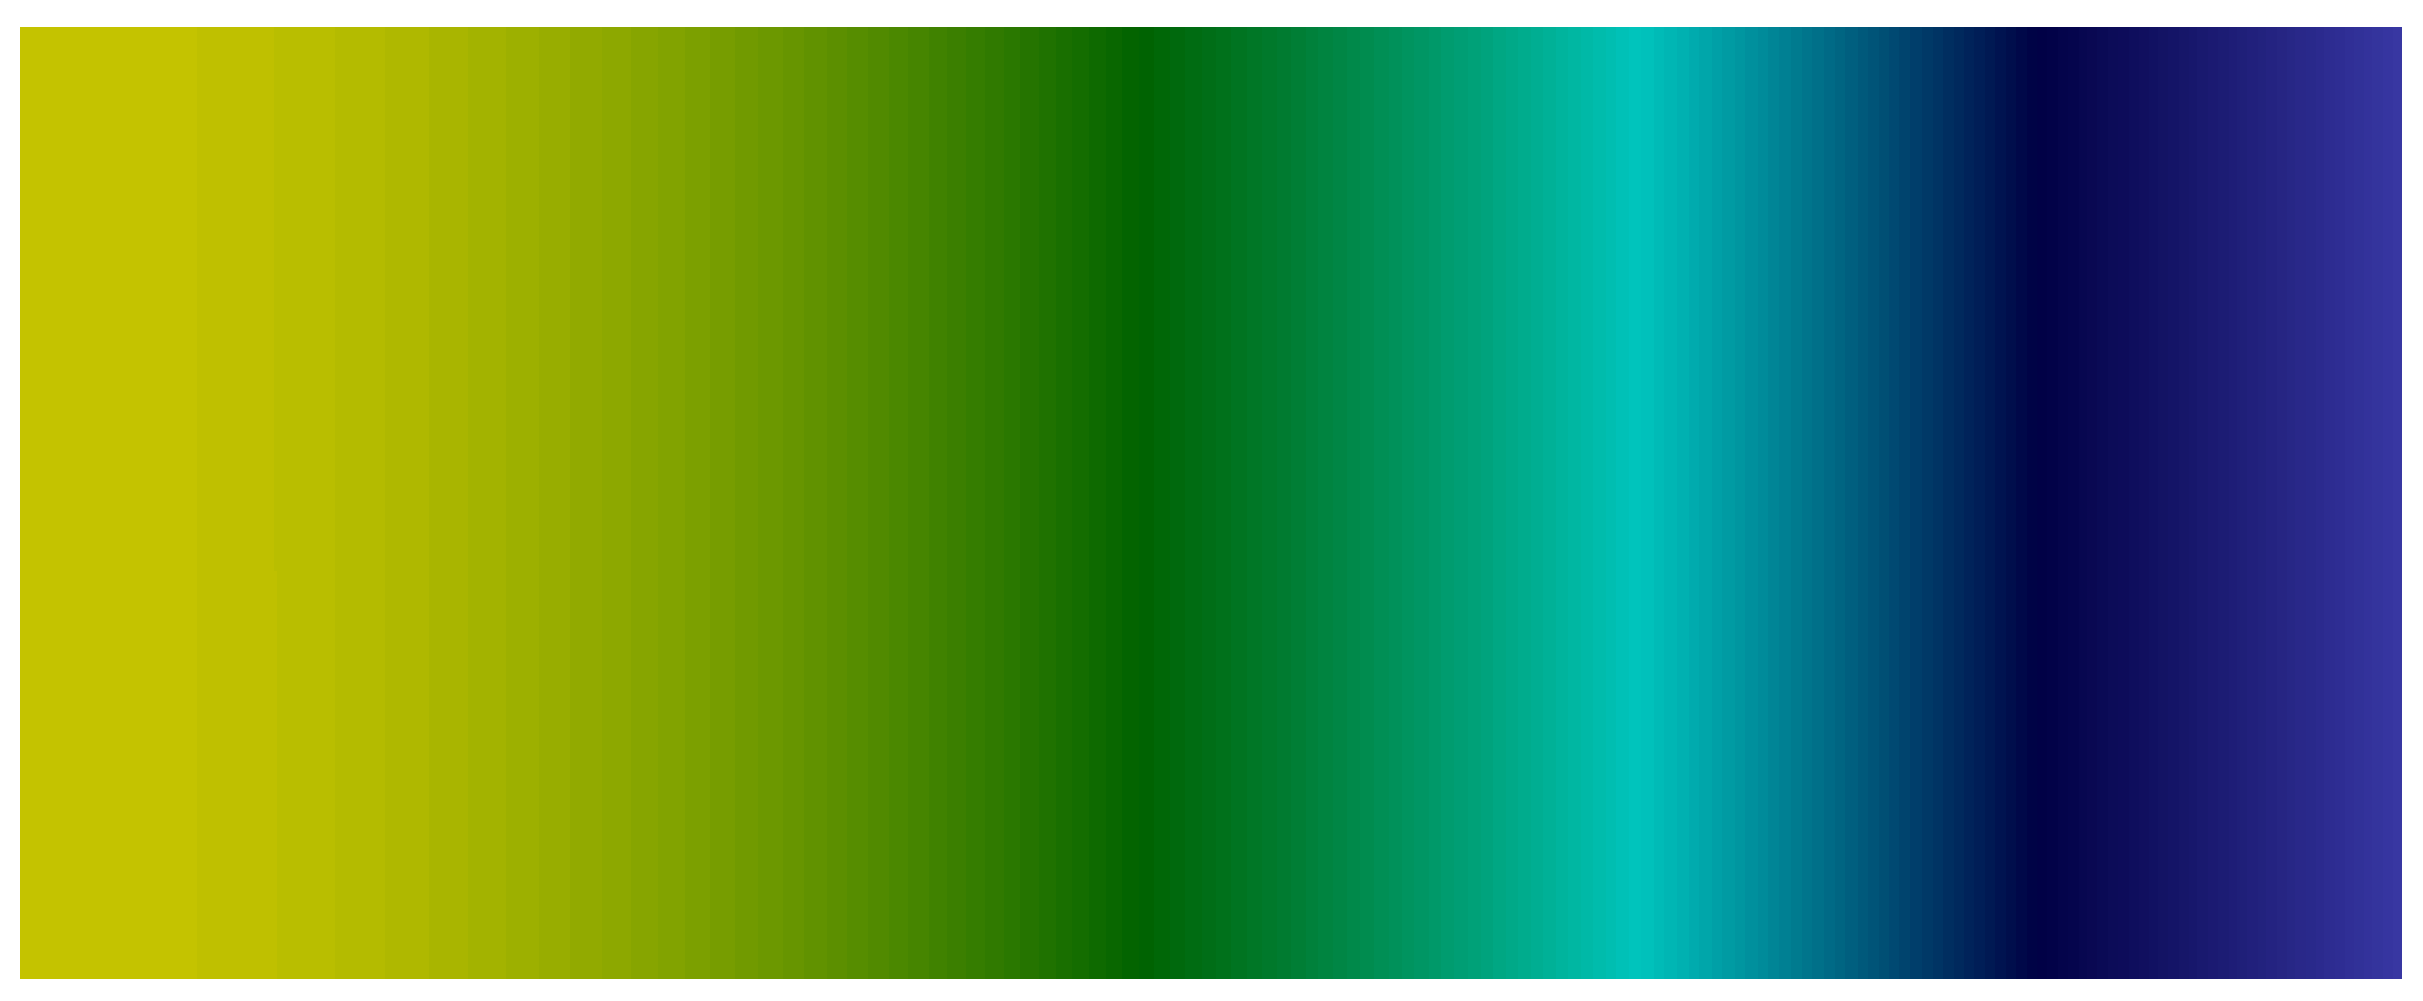
\includegraphics[width=80mm]{t299}\label{Fig:mandel_t_299}}
		\\
		\subfloat[]{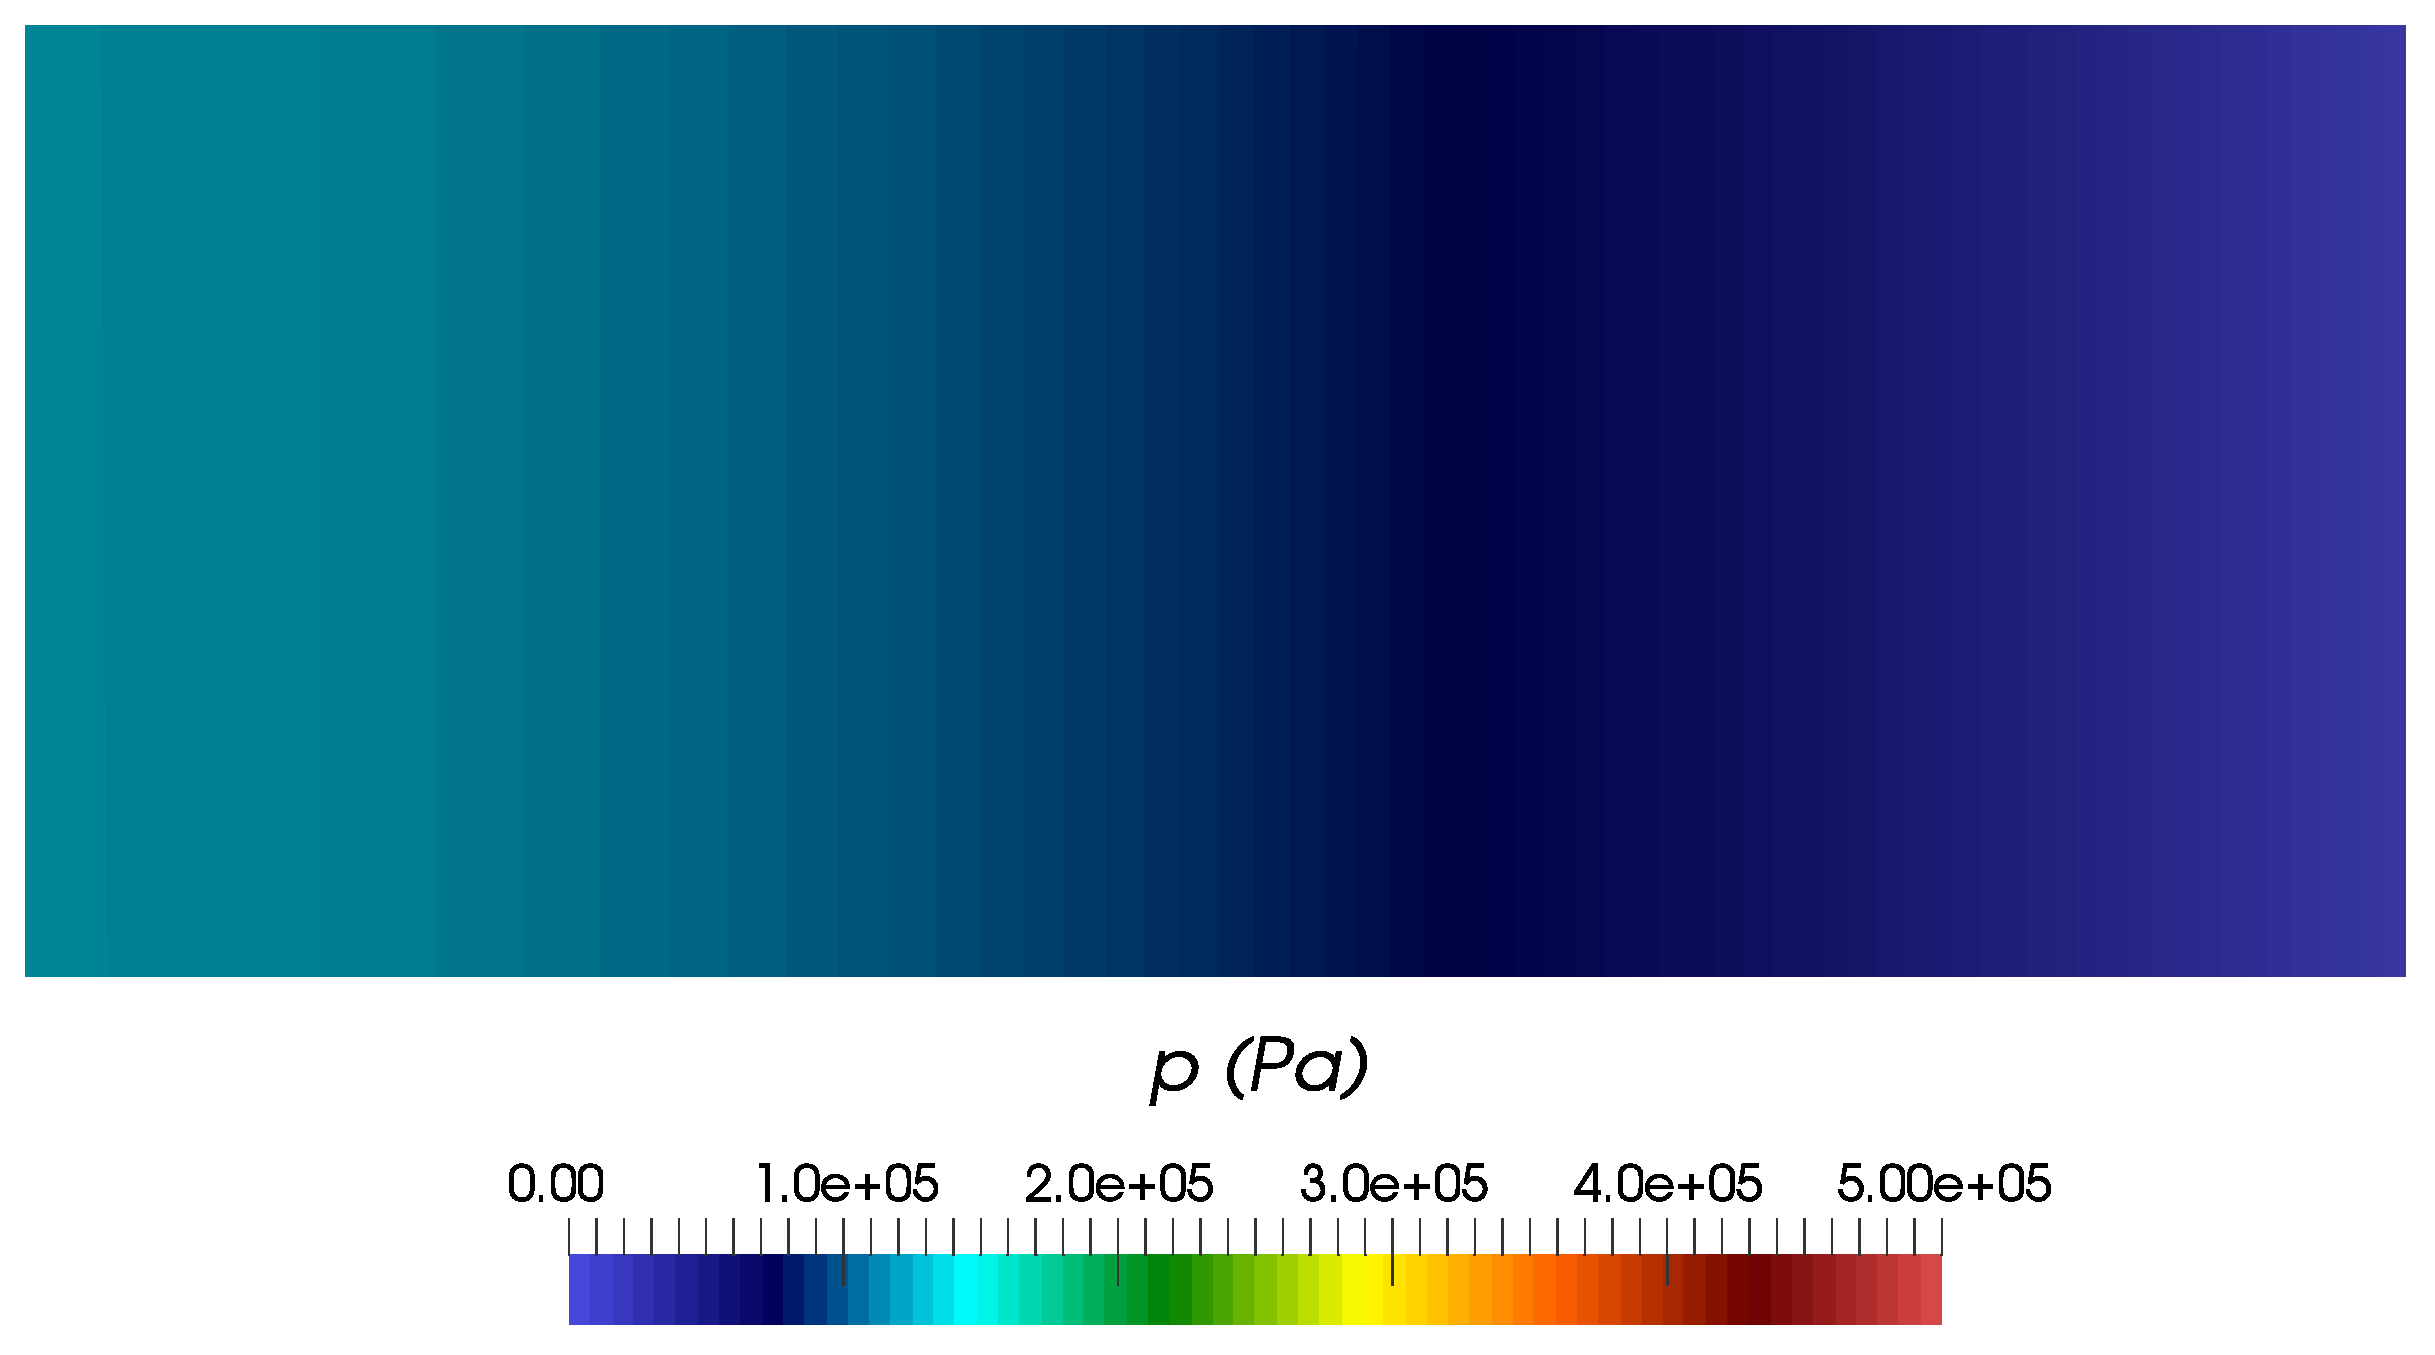
\includegraphics[width=80mm]{t599}\label{Fig:mandel_t_599}}
		\caption{Pressure profile at different stages (\ref{Fig:mandel_t_9}) $t=0.1s$, (\ref{Fig:mandel_t_199}) $t=2s$, (\ref{Fig:mandel_t_299}) $t=3s$, and (\ref{Fig:mandel_t_599}) $t=6s$). At very early stages, the pressure rises  rapidly in response to the instantaneous loading, then gradually decays to zero. %while drops until it nearly vanishes.
		}
		\label{Fig:mandel_snapshots}
	\end{figure}

A comment on Mandel's problem follows here.	
It is true that this problem is a typical poroelastic problem. However, it would somehow repeat our second verification example (see Section 4.2) where the porous flow is coupled with the porous medium's displacement. The example in Section 4.2 solved by Detourney and Cheng [56] has been used in a few works, e.g., [11][57], to verify the solution to the poroelastic response of a pressurized borehole. For these reasons, we preferred not to include Mandel's problem in the manuscript. 
		
\clearpage

    \review{
    	The phase field method for hydraulic fracture modeling is indeed successfully verified through semi-analytical solutions in other researchers' work. However, this does not indicate all the models utilizing the phase field method can be correctly verified through the semi-analytical solutions. The authors have to demonstrate that the model in this paper can match the semi-analytical solutions. I cannot understand why the authors think it is not necessary to verify their model just because the verification of the same method is already performed by other researchers.}  	
  	
 % 	\todo[inline, author=YS]{Can we say these two points: 1. Compressible fluids are very different from incompressible ones. The only existing asymptotic solutions are for incompressible. We verified our solution with Wang's results. 2. We did try to compare our results with KGD as much as we could. The fracture length result was fine, but still too much off to show in the manuscript.}
  	
	\bigskip
%	\todo[inline,author=YS]{We need to start with the POINT. If there are multiple points, then number them.}
%To best of our knowledge, there exist {only a few} studies focusing on the verification of phase field method with asymptotic analytical solutions \cite{chukwudozie2016application, wilson2016phase}. As the phase field part of our method is fully based on the literature and very similar to the verified models, the authors did not plan to repeat such verification\todo[author=YS]{Bad response. This kind of statement only escalates the conflict.}.

Let us reiterate that our model for CO$_2$ treats it as a \emph{compressible} fluid. None of existing papers that models fracturing with compressible CO$_2$ verifies with asymptotic semi-analytical solutions with hydraulic fracturing, the latter of which are based on an \emph{incompressible} assumption of the fluid. Compressible fluids behave very differently from incompressible ones.

For verifying our model, we have not only checked the convergence of the discretization parameters for space and time, but also compared our examples in the manuscript against various solutions: the Hubbert-Willis (H-W) solution [60], the Haimson-Fairhurst (H-F) solution [61], the Sneddon and Lowengrub solution [58], and the Detourney and Cheng solution [56].




%In the following, we provide a brief study on how much our phase field model can match the asymptotic solutions through a KGD model. We did try a few examples to verify our model for a toughness-dominated regime (K-vertex), and we saw our results can match to analytical solutions up to a limited degree.
%To best of our knowledge, the only existing asymptotic solutions are for incompressible fluids. Compressible fluids are expected to behave very differently from incompressible ones. This fact might explain why our results cannot fit properly to asymptotic solutions. However, note that among a very few existing literature for incompressible gas flow, we verified our examples in the manuscript by the Hubbert-Willis (H-W) solution [60], Haimson-Fairhurst (H-F) solution [61], Sneddon and Lowengrub [58], and  Detourney and Cheng [56]. Also, the results are independent of spatial and temporal discretization.


In response to the reviewer's request, we have reached out by applying our compressible formulation to the equation of state of water [R.~T.~Fernandez. Natural Convection from Cylinders Buried in Porous Media. PhD thesis, University of California; 1972] for a fracturing problem in the toughness-dominated regime (K-vertex), in order to compare our solution with the KGD model [J. Geertsma and F. De Klerk, A rapid method of predicting width and extent of hydraulically induced fractures, Journal of Petroleum Technology 21 (12) (1969) 1–571].
%We follow a toughness-dominated regime to verify our model through KGD solutions. 
%When the toughness is very big, it is again the solution by Sneddon and Lowengrub [58], which we have already verified with in the manuscript.
%\emph{First} we assume the fracture toughness is very big, which is nothing else than Section 4.3, where we present the classical example solved by Sneddon and Lowengrub [58]. In this example, we compute the opening displacement of a static line crack with our proposed model, and compare it with the aperture profiles by the Sneddon's analytical solutions. \emph{Second}, 
%With a related toughness we let the crack propagate and compare the numerical results with KGD model [J. Geertsma, F. De Klerk, et al., A rapid method of predicting width and extent of hydraulically induced fractures, Journal of Petroleum Technology 21 (12) (1969) 1–571]. We  tried to model water with our formulation by changing EOS to that of water, and related material parameters. 
The parameters are given in Table \ref{Tab:asymptotic_input}.
Figure \ref{Fig:KGD_width_water} plots the evolution of the maximum fracture aperture of our numerical results and the KGD analytical solution. A good agreement is observed.
Nevertheless, the fracture length evolution and the injection pressure do not agree well (not shown). This might be due to the over-extrapolation of the formulation to a fracturing fluid (water) that the formulation was not intended to model.

\begin{table}[htbp]
	\centering
	\caption{Parameters for the comparison of KGD solution using the equation of state of water (a compressible formulation).}
	\begin{tabular}{l c c c}
		\hline 
		Parameters & symbol & unit& value \\
		\hline 
		Young's modulus & $E$ &MPa&  6$\times 10^{3}$\\
		Poisson's ratio & $\nu$ &$-$&  0.34\\
		Critical energy release rate & $g_c$ &MPa$\cdot$mm&  0.306\\
		%Regularization length scale & $\ell$ &$-$&  1.6$\times 10^{-4}$\\
		Biot coefficient & $\alpha$ &$-$&  0.85\\
		Porosity & $\phi$ &$-$&  0.01\\
		Initial permeability & $k_0$ &mm$^2$&  1$\times 10^{-12}$\\
		Dynamic viscosity of water & $\mu$ & MPa$\cdot$s& 7.9$\times 10^{-3}$\\
		%Bulk modulus of fluid & $k_f$ &$KN/mm^2$&  0.625$ \times 10^{3}$\\
		% Bulk modulus of rock & $k_s$ &$KN/mm^2$&  10$ \times 10^{3}$\\
		Initial pressure & $p_0$ &MPa& 0.1\\
		%Rock's tensile strength & $\sigma_T$ &MPa& 11\\
		%Maximum principal stress & $\sigma_1$ &MPa&  1\\
		%Minimum  principal stress & $\sigma_3$ &MPa&  1\\
		Final time &$t_f$ & s &  500\\
		Flow rate &${\bm{v}} \cdot n$ & mm$^2$/s & 5\\
		\hline     
	\end{tabular}
	\label{Tab:asymptotic_input}
\end{table}

%Some comments on verification with asymptotic solutions are given here:  \emph{1) Compressible fluids are very different from incompressible one. The existing KGD solutions can match our model up to a limited degree. This might be due to the fact that our model is for compressible gas flow, while KGD models are for incompressible fluid; \emph{2)}  We did try to compare our results with KGD as much as we could. The fracture length result was fine, but still too much off to show in the manuscript;  \emph{3)} Please also note that {only a few} studies have been focusing on the verification of phase field method with asymptotic analytical solutions [43][50]. Thus, there is still room left for further investigations.}

%\deleted[id=MM]{{This example is also studied in Section 4.5, CO$_2$ driven fracture.}
%{Here, we closely follow our example in Section 4.5, CO$_2$ driven fracture, and use the same input data and boundary conditions. 
%The sample is discretized into $18,568$ three-noded triangular elements so that the mesh size $h=0.58~$mm is obtained while we set $\ell=1.6~$mm. Note that the flow rate $Q_g$ and simulation time $t_f$ are $1.6\times10^{-5}~ \text{m}^2/\text{s}$ and $2.545\times 10^{-2}$s, respectively.}
%Figures \ref{Fig:KGD_length}{-}\ref{Fig:KGD_pressure}
%\ref{Fig:KGD_width}, and \ref{Fig:KGD_pressure} demonstrate the comparison of our numerical results from Section 4.5 with KGD analytical solutions \cite{geertsma1969rapid} for fracture length, maximum fracture opening width, and wellbore pressure, respectively. In Figure \ref{Fig:KGD_length}, a relatively good agreement is obtained for the fracture length. For wellbore pressure, however, in Figure \ref{Fig:KGD_pressure} we observe the pressure is noticeably bigger than the KGD solution. \todo[author=YS]{What does it have to do with breakdown here? Vahid: Removed.} Also, the maximum fracture aperture in Figure \ref{Fig:KGD_width} is computed within the same order, but still bigger than the KGD solution. Also see Figure \ref{Fig:width_length_diffrentTime} for fracture width opening profile at different stages. In brief, our model can match to the existing KGD solutions for incompressible fluids up to a limited degree. This might be due to the fact that our model is for compressible gas flow, and this will make a huge difference.}
%\begin{figure}[htbp]
%	\centering
	%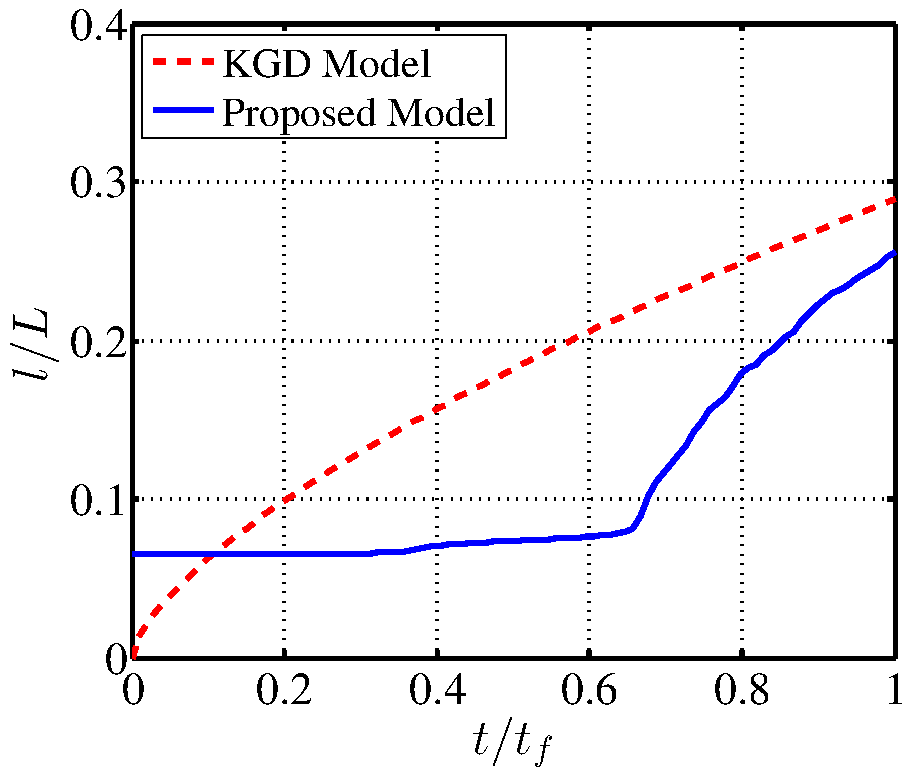
\includegraphics[width=0.7\textwidth]{LENGHT_KGD}
%	\caption{\deleted[id=MM]{Verification of fracture length for a toughness-dominated regime with KGD analytical solution \cite{geertsma1969rapid}. A relatively good agreement is observed.}}
%	\label{Fig:KGD_length}
%\end{figure}
%\begin{figure}[htbp]
%	\centering
	%\includegraphics[width=0.7\textwidth]{width_KGD}
%	\caption{\deleted[id=MM]{Verification of maximum fracture width for a toughness-dominated regime with KGD analytical solution \cite{geertsma1969rapid}.}}
%	\label{Fig:KGD_width}
%\end{figure}
%\begin{figure}[htbp]
%	\centering
	%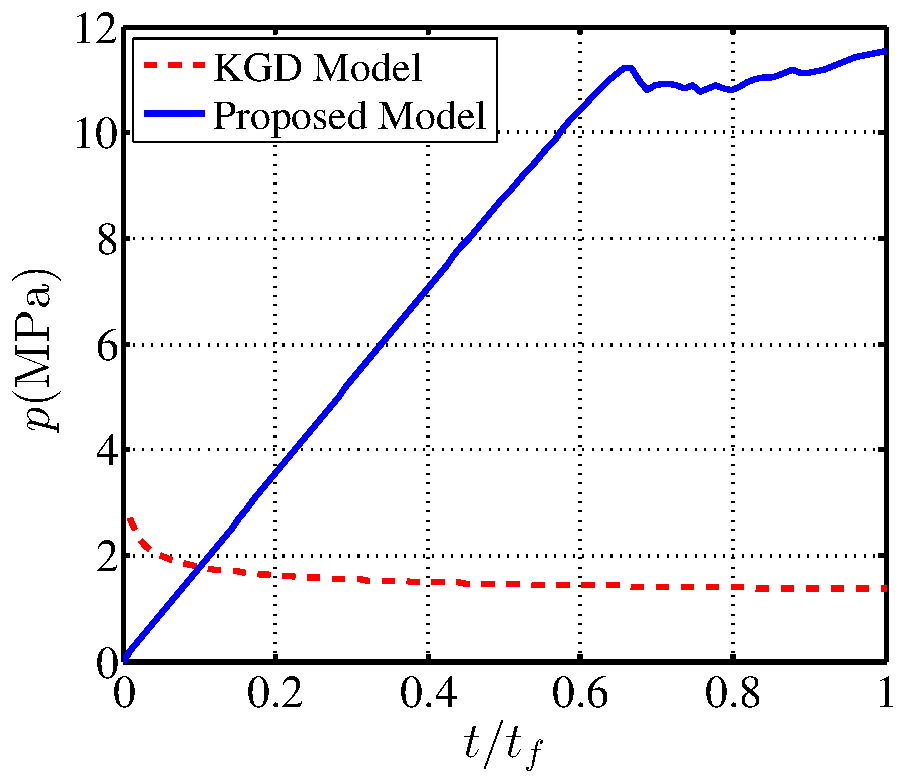
\includegraphics[width=0.8\textwidth]{pressure_KGD}
%	\caption{\deleted[id=MM]{Verification of injecting pressure for a toughness-dominated regime with KGD analytical solution \cite{geertsma1969rapid}.}}
%	\label{Fig:KGD_pressure}
%\end{figure}
%\todo[inline,author=YS]{Why in Figure \ref{Fig:width_length_diffrentTime} there is no comparison with KGD?\\Vahid: With KGD we can have the maximum crack width. Here, we show the opening profile along the crack. Thus, a comparison cannot be made (we already did in Figure \ref{Fig:KGD_width}). This is one typical poroelastic response though. It shows the right trend of increasing opening.\\ YS: I believe we have more than just the maximum crack width. Didn't KGD also solve for the opening profile?
%\\MM: KGD can only give you the maximum width of the crack that will occur in the borehole. }
%\begin{figure}[htbp]
%	\centering
	%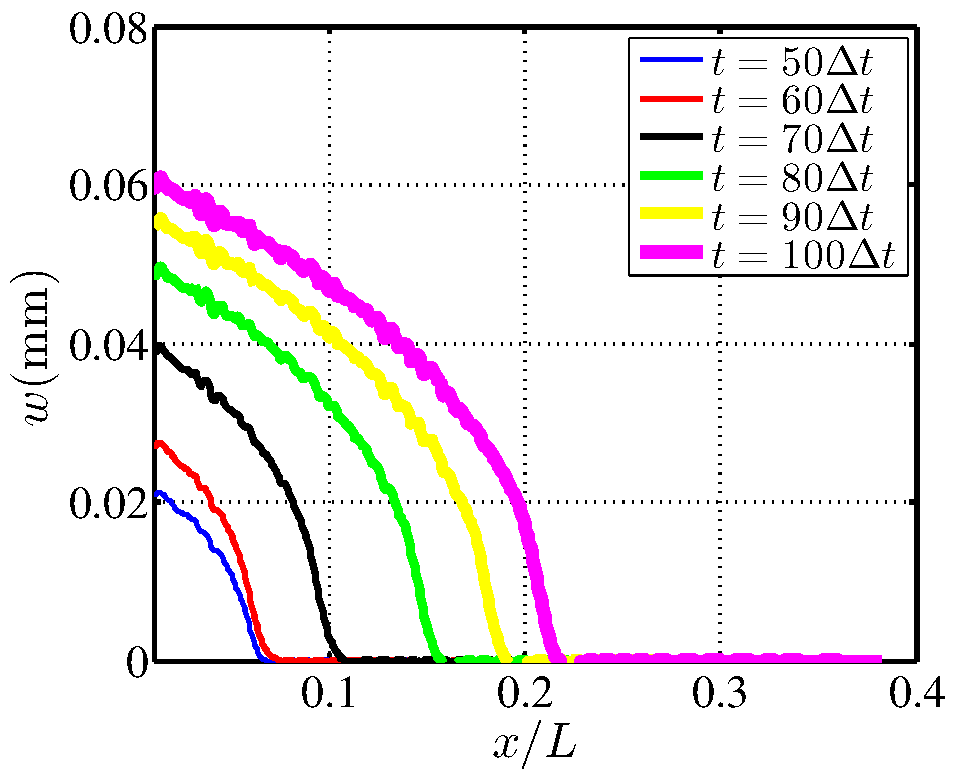
\includegraphics[width=0.7\textwidth]{width_length_diffrentTime}
	%\caption{\deleted[id=MM]{The fracture opening profile at different stages.}}
%	\label{Fig:width_length_diffrentTime}
%\end{figure}
%\deleted[id=MM]{In the following, we aim to see if changing $\rho-p$ relation can lead into a behavior closer to KGD solutions. For this purpose, we attempt to model some fictitious less-compressible gas by changing EOS. We multiply EOS by different coefficients \dots, and plot the fracture length in Figure \ref{Fig:KGD_length_diff_Coeff}. We see nearly no difference in these profiles. Thus, we can conclude that the solution is not heavily sensitive to the change in EOS.}
%\begin{figure}[htbp]
%	\centering
	%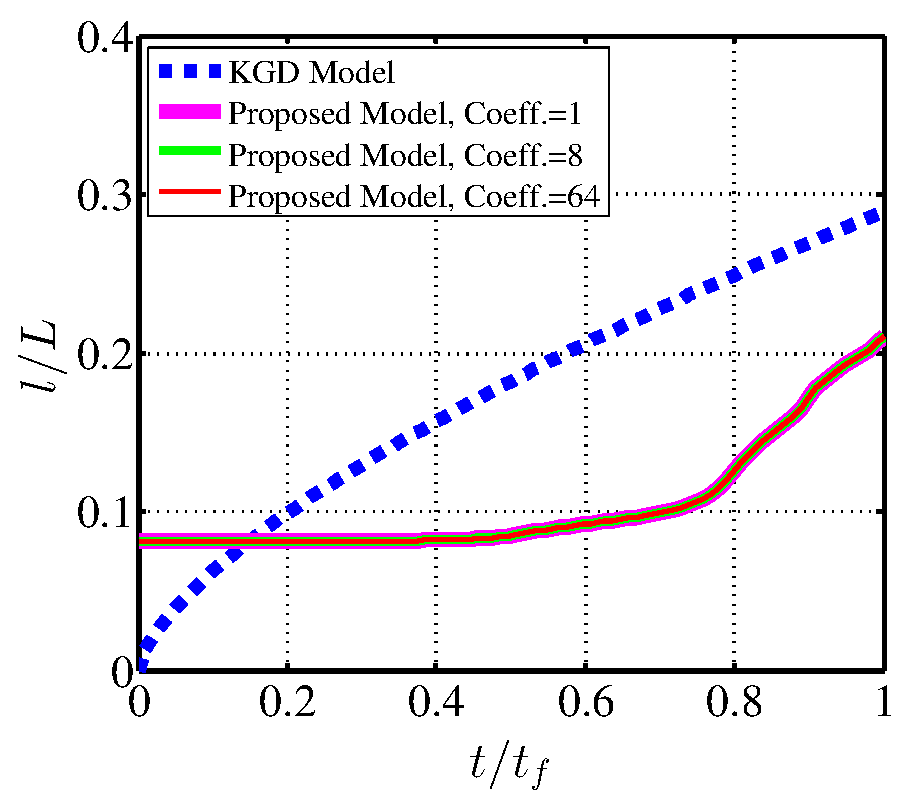
\includegraphics[width=0.7\textwidth]{differentcoef_length}
%	\caption{\deleted[id=MM]{Testing the proposed model with KGD solutions using semi-incompressible artificial gas \dots}}
%	\label{Fig:KGD_length_diff_Coeff}
%\end{figure}
%\paragraph{\deleted[id=MM]{modeling water with our formulation}}\deleted[id=MM]{ We also tried to model water with our formulation by changing EOS to that of water, and related material parameters. Figures \ref{Fig:KGD_length_water}-\ref{Fig:KGD_width_water} illustrates the comparison of our numerical results with KGD analytical solution for fracture length, maximum fracture opening width, and wellbore pressure, respectively. A good agreement is observed for the opening.}
%\begin{figure}[htbp]
%	\centering
	%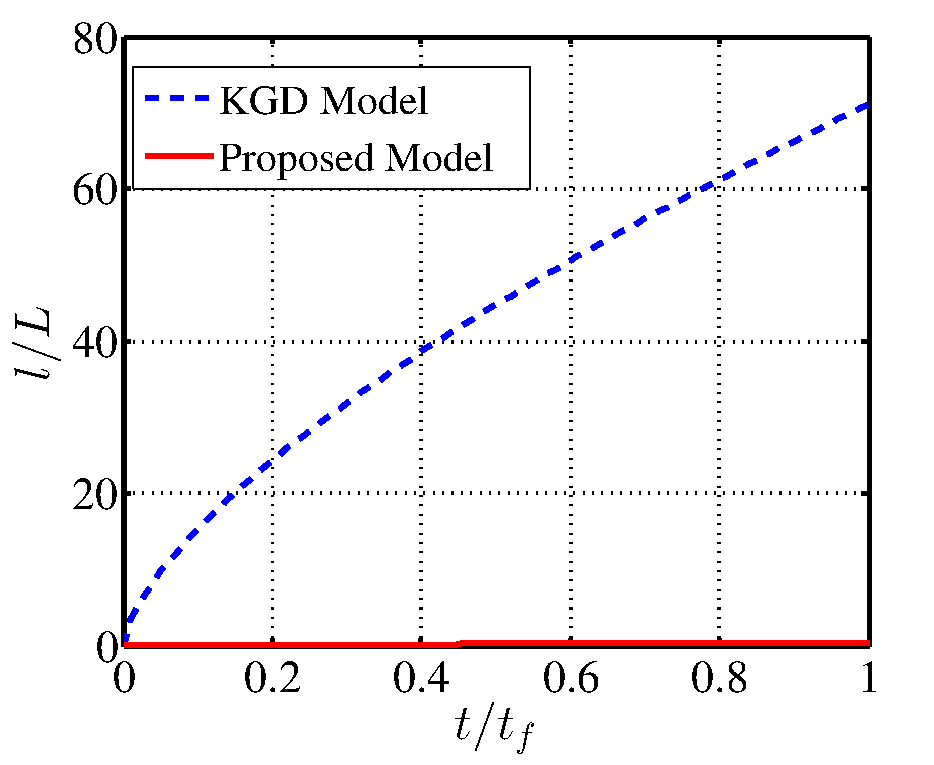
\includegraphics[width=0.7\textwidth]{LENGTH_KGD_watter}
%	\caption{\deleted[id=MM]{Verification of fracture length for a toughness-dominated regime with KGD analytical solution \cite{geertsma1969rapid}.}}
%	\label{Fig:KGD_length_water}
%\end{figure}
\begin{figure}[htbp]
	\centering
	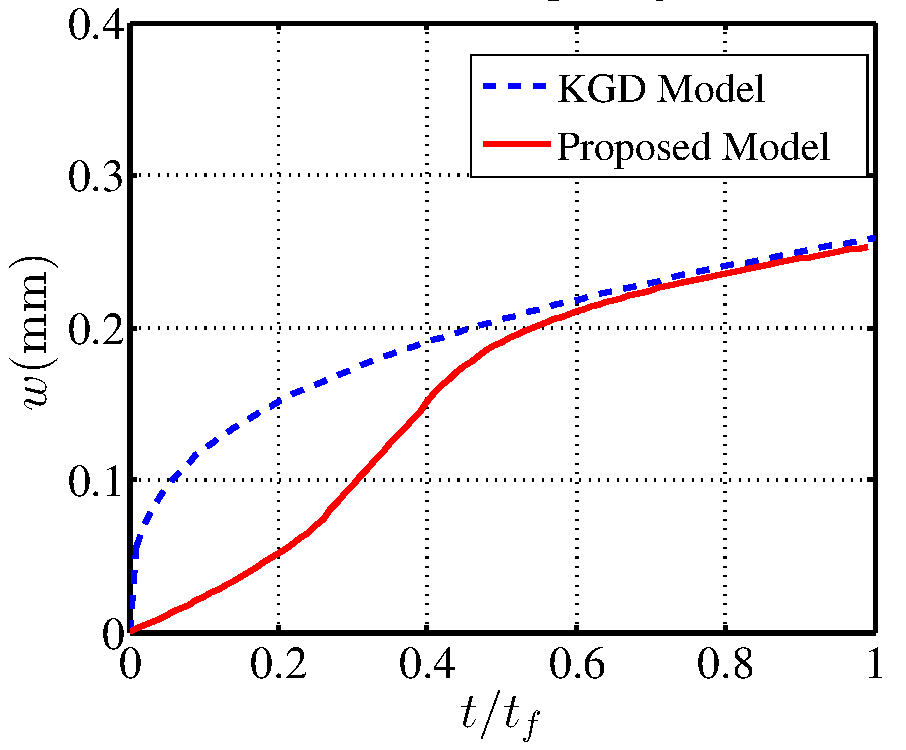
\includegraphics[width=0.7\textwidth]{Width_KGD_water}
	\caption{Verification of maximum fracture width for a toughness-dominated regime with KGD analytical solution [Geertsma and de Klerk, 1969].}
	\label{Fig:KGD_width_water}
\end{figure}
%\begin{figure}[htbp]
%	\centering
%	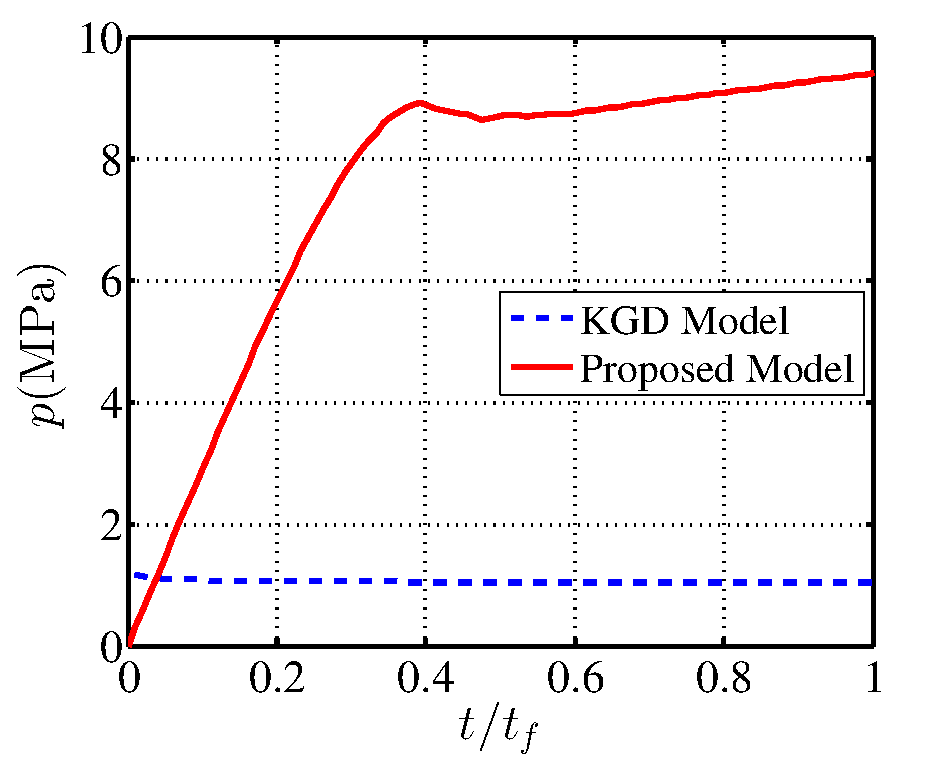
\includegraphics[width=0.7\textwidth]{Pressure_KGD_water}
%	\caption{\deleted[id=MM]{Verification of injecting pressure for a toughness-dominated regime with KGD analytical solution \cite{geertsma1969rapid}.}}
%	\label{Fig:KGD_pressure_water}
%\end{figure}

%\deleted[id=MM]{A comment on verification with asymptotic solutions is given here. The existing KGD solutions can match our model up to a limited degree. This might be due to the fact that our model is for compressible gas flow, while KGD models are for incompressible water. Please also note that only a few studies have been focusing on the verification of phase field method with asymptotic analytical solutions} \cite{chukwudozie2016application,wilson2016phase}. \deleted[id=MM]{Thus, there is still room left for further investigations.}

%\clearpage
\bigskip
    \review{2. Regarding Question 2:
    	All the given three references assume that grains are incompressible, which could be used approximately for soil. But this study is not about soil, it is about reservoir rock. There would not be too many people in the petroleum industry using this assumption in simulations.}
    	\bigskip
    	
	It is true that including more complex assumptions for grains can lead to a more realistic model. However, we can cite a few works in which the grains for the reservoir are assumed incompressible: [M.~Sheng, G.~Li, S.~N.~Shah, X.~Jin, Extended finite element modeling of multi-scale flow in fractured shale gas reservoirs, in: SPE Annual Technical Conference and Exhibition, Society of Petroleum Engineers, 2012, pp. SPE-159919-MS] and [A.~Verruijt, Theory and Problems of Poroelasticity, 2013]. Thus, we believe the assumption adopted here is not too much out of the norm.
	\bigskip

    \review{3. Regarding Question 3: The discretization of the weak form is for solid part of a poroelastic model. The fluid flow part is entirely ignored.}
	\bigskip
	
In Appendix A.2 of the first revision, the discretization for fluid part was already provided. Moreover, we added one extra reference at the beginning of Appendix A for the implementation details. %Note that for the phase field part, we do not solve for $p$.

	\bigskip
    \review{In summary, the sequential coupling through volume strain is not correct; the model is not verified correctly, the correctness of the numerical model presented here is unknown.}
 \bigskip
 
We hope our response has clarified most of the issues.

%\bigskip


%\clearpage
%\todo[inline,author=YS]{Why not use reference numbers in the manuscript? Then we do not need to have a bibliography here, or just those not cited in the manuscript.\\Vahid: I removed the bibliography. I still do not know how to export the same numbers as they are in the manuscript \dots\\YS: Just manually input the numbers.\\MM: In my opinion, It's not a good idea, because we have some new references here. For example, we will have two references one in this way. Unless we start our reference number here from 64 (we have 63 references in our manuscript).  }

%\bibliographystyle{elsarticle-num}
%\nobibliography{ref.bib}
%\bibliographystyle{elsarticle-num}
%\bibliography{../Revision/ref}
\end{document}